\documentclass[upright, contnum]{umemoria}
\depto{Departamento de Ingeniería Eléctrica}
\author{Rodrigo Javier Pérez Dattari}
\title{Interactive Learning with Corrective Feedback for Continuous-Action Policies based on Deep Neural Networks}
\auspicio{FONDECYT Projecto 1161500.}
\date{2018}
\guia{Javier Ruiz del Solar}
\carrera{Magíster en Ciencias de la Ingeniería, Mención Eléctrica}
\carreraeng{Master of Engineering Sciences in Electrical Engineering}
\memoria{Tesis para optar al Grado de \break  Magíster en Ciencias de la Ingeniería, Mención Eléctrica\break \break
Memoria para optar al Título de Ingeniero Civil Eléctrico}
\comision{Carlos Celemin}

\usepackage{lipsum}

\usepackage[latin1]{inputenc}
\usepackage[T1]{fontenc}
\usepackage{color}

\newcommand{\note}[1]{\color{red}\textbf{{#1}}\color{black}}

\begin{document}

\frontmatter
\maketitle

\begin{abstract}

\end{abstract}

\begin{abstract_eng}
Deep Reinforcement Learning (DRL) has become a powerful methodology to solve complex decision making problems. However, DRL has several limitations when used in real-world problems (e.g., robotics applications). For instance, long training times are required and cannot be accelerated in contrast to simulated environments, and reward functions may be hard to specify/model and/or to compute. Moreover, the transfer of policies learned in a simulator to the real-world has limitations (reality gap). On the other hand, machine learning methods that rely on the transfer of human knowledge to an agent have shown to be time efficient for obtaining well performing policies and do not require a reward function. In this context, we analyze the use of human corrective feedback during task execution to learn policies with high-dimensional state spaces, by using the D-COACH framework, and we propose new variants of this framework. D-COACH is a Deep Learning based extension of COACH (COrrective Advice Communicated by Humans), where humans are able to shape policies through corrective advice. The enhanced version of D-COACH, which is proposed in this paper, largely reduces the time and effort of a human for training a policy. Experimental results validate the efficiency of the D-COACH framework in three different problems (simulated and with real robots), and show that its enhanced version reduces the human training effort considerably, and makes it feasible to learn policies within periods of time in which a DRL agent do not reach any improvement.
\end{abstract_eng}


\begin{dedicatoria}
A mi abuelo Ernesto.
\end{dedicatoria}

\begin{thanks}

\end{thanks}

\cleardoublepage
\tableofcontents
\cleardoublepage
\listoftables
\cleardoublepage
\listoffigures

\mainmatter

\chapter{Introduction}
\section{Motivation and Problem Statement}
In  recent years, outstanding results in complex decision-making problems have been obtained with Deep Reinforcement Learning (DRL). State-of-the-art algorithms have solved problems with large state-action spaces, such as playing Atari games \cite{atari}, beating the world champion in GO \cite{Silver2016} or defeating a top professional player in StarCraft II \cite{alphastarblog}, along with low level simulated continuous control tasks in environments such as the ones included in the OpenAI Gym \cite{brockman2016openai} and the DeepMind Control Suite \cite{tassa2018deepmind}. 

Nevertheless, in robotic problems, DRL is still limited in applications with real-world problems \cite{Gu2017}. Most of the tasks that have been successfully addressed with DRL have two common characteristics: 1) they have well-specified reward functions, and 2) they require large amounts of trials, which means long training periods (or powerful computers) to obtain a satisfying behavior. These two characteristics can be problematic in cases where 1) the goals of the tasks are poorly defined or hard to specify/model (reward function does not exist), 2) the execution of many trials is not feasible (real systems case) and/or not much computational power or time is available, and 3) sometimes additional external perception is necessary for computing the reward/cost function.

In this regard, the transfer of knowledge learned in a simulator to the real-world is a typical solution. However, the mismatch between the virtual and real environment, known as ``Reality Gap``, is often problematic \cite{koos2013transferability}. This results in agents that do not perform at their best in the real-world. Thus, it would be preferable to learn/fine-tune policies directly in the real-world.

In contrast, Machine Learning methods that rely on transfer of human knowledge, Interactive Machine Learning (IML) methods, have shown to be time efficient for obtaining good performance policies and may not require a well-specified reward function; moreover, some methods do not need expert human teachers for training high performance agents \cite{akrour2011preference,Knox:2009:ISA:1597735.1597738,Celemin2018AnInteractive}. In previous years, IML techniques were limited to work with low-dimensional state spaces problems and to the use of function approximation such as linear models of basis functions (choosing a right basis function set was crucial for successful learning), in the same way as Reinforcement Learning (RL). But, as DRL have showed, by approximating policies with Deep Neural Networks (DNNs) it is possible to solve problems with high-dimensional state spaces, without the need of feature engineering for preprocessing the states. If the same approach is used in IML, the DRL shortcomings mentioned before can be addressed with the support of human users who participate in the learning process of the agent.

Therefore, in this work we study the use of human corrective feedback during task execution to learn DNN policies in state spaces of low and high dimensionality in continuous action problems (which is the case for most of the problems in robotics).

In this context, this thesis proposes an alternative Interactive Machine Learning strategy for training Deep Neural Network policies based on human corrective feedback, with a method called Deep COACH (D-COACH). Deep Learning is combined with the COrrective Advice Communicated by Humans (COACH) framework, in which non-expert humans shape policies by correcting the agent’s actions during execution. The D-COACH framework has the potential to solve complex problems without much data or time required. Experimental results validated the efficiency of the proposed framework in simulated and real-world platforms, with state spaces of low and high dimensionality, showing the capacity to successfully learn policies for continuous action spaces. 

Three variations of D-COACH are introduced:

\begin{enumerate}
    \item \textbf{Offline state representation learning (D-COACH)}
    \item \textbf{ONline state representation learning (D-COACH ON)}
    \item \textbf{Memoryful ONline state representation learning (D-COACH MON)}
\end{enumerate}

D-COACH and D-COACH ON assume that the agents interact in fully-observable environments. As a consequence, they make decisions solely based on what they are observing on that precise moment. There is no difference between these two approaches in problems with low-dimensional states. A fully connected network policy is interactively trained during task execution with human corrective feedback. Nevertheless, in high-dimensional state problems D-COACH ON enhances the methodology proposed in D-COACH. In both approaches a convolutional autoencoder is added to the network architecture for state dimensionality reduction. In the D-COACH formulation, a demonstration session is required at the beginning of the training process for tuning the weights of the autoencoder. After that, a fully connected network policy is linked to the output of the encoder layers (latent space of the autoencoder), and is trained interactively, in the same way as in the low-dimensional state case. In contrast, D-COACH ON eliminates the need of demonstration sessions and trains the policy and the autoencoder simultaneously, sharing the convolutional layers (encoder) between both networks. This reduces the time and effort of the human for teaching a policy.

D-COACH MON assumes that the agents interact in partially-observable environments, which is true in many real-world scenarios, and tries to cover a subset of these problems. Memory is added to the agents by using recurrent layers in the network architectures in order to obtain well performing policies in problems where past observations contain crucial information about the current state of the agent. As in D-COACH ON, everything is learned online, without the need of a demonstration session. 

Throughout this thesis, we give special emphasis to studying the use of policies parameterized with Convolutional Neural Networks (CNNs) for solving problems with high-dimensional state spaces, such as raw pixels from an image. CNNs give agents the possibility to build rich state representations of the environment without feature engineering on the side of the designer (which was always necessary in classical RL). These properties can be very useful in robotics, since it is common to find applications with high-dimensional observations, such as RGB images. Giving robots the ability to learn from such high-dimensional data will allow to scale up the complexity of what robots are able to do. All of the proposed variations of D-COACH have as common denominator the study of CNNs,  seeking to exploit their properties in the best possible way. 

\section{Objectives}
\subsection{General Objective}
The general objective of this thesis is to develop and validate an algorithm that exploits the advantages of combining deep learning with human corrective feedback for learning policies when solving sequential decision-making problems in robotics. 

\subsection{Specific Objectives}

\begin{itemize}
    \item Study the state-of-the-art of robot learning algorithms for solving sequential decision-making problems.
    \item Propose and implement an algorithm that, by using deep neural networks policies, allows robots to learn to solve tasks in continuous-action domains from low-dimensional and high-dimensional states using online human corrective feedback. 
    \item Validate the proposed algorithm with tasks using simulated and real platforms.
    \item Propose and validate a variation of the algorithm to solve problems with partially observed environments.
\end{itemize}

\section{Hypothesis}
Human corrective feedback can be used to learn well performing deep neural network policies. As a consequence, an algorithm of this kind will effectively inherit the learning properties of using human corrective feedback and the function approximation properties of deep neural networks. Combining both approaches will result in a time-efficient and reward function free learning algorithm capable of solving problems using complex observations, such as raw pixels from an image.

\section{Outline}
This thesis is divided in six chapters.

\begin{itemize}
    \item \textbf{Chapter 2} presents the theoretical framework of this work. Both the areas of sequential decision-making and deep learning are revised in order to use them as baselines for the development of the thesis.
    \item \textbf{Chapter 3} introduces D-COACH. The ideas taken from the COACH framework are discussed and the formulation of D-COACH is presented. This approach is validated using simulated and real-world platforms.
    \item \textbf{Chapter 4} proposes an enhanced variation of D-COACH introduced in Chapter 2 (D-COACH ON), tackling one of its main shortcomings. This new version of the algorithm is able to learn policies from scratch in problems with high-dimensional state spaces in one learning step, while the previous version of D-COACH had an extra offline learning step.
    \item \textbf{Chapter 5} introduces a variation of D-COACH that adds memory to the agents (D-COACH MON) in order for them to solve tasks in partially observable environments. In contrast, Chapters 3 and 4 assume that the environments are fully observable, which is not true in many real-world scenarios.
    \item \textbf{Chapter 6} gathers the conclusions and the future work of this thesis.
\end{itemize}
\chapter{Theoretical Framework}
\section{Machine Learning}

Machine Learning (ML) is a discipline that studies ways of finding patterns in data by learning from experience. What this mean, is that an algorithm in charge of accomplishing an specific task is able to progressively improve its performance (learn) by comparing its output with data (experience) in a way that indicates how good/bad is doing. If the algorithm is doing good, then the learning process is finished. If is not doing so good, then the algorithm updates its parameters to match (if possible) its output with what is expected.   
\subsection{Deep Learning}

\subsubsection{Autoencoder}

\section{Policy Learning}
\note{POLICY DESCRIPTION}
\subsection{Reinforcement Learning}
\subsubsection{Deep Reinforcement Learning}
\subsection{Learning from Demonstration}
\subsubsection{The Correspondence Problem}
\subsection{Interactive Learning}
\subsubsection{Evaluative Feedback}
\subsubsection{Corrective Feedback}
\section{Function Approximation}
\subsection{Linear Model of Basis Functions}
\subsection{Artificial Neural Networks}
\section{COrrective Advice Communicated by Humans (COACH)}
\chapter{Introducing Deep Neural Networks into the COACH Framework}
In this chapter, we propose to extend the use of human corrective feedback during task execution to learn policies with state spaces of low and high dimensionality in $\text{continuous-action}$ problems (which is the case for most of the problems in robotics) using deep neural networks.

 We combine Deep Learning (DL) with the corrective advice based learning framework called COrrective Advice Communicated by Humans (COACH) \cite{Celemin2018AnInteractive}, thus creating the Deep COACH (D-COACH) framework. In this approach, no reward functions are needed and the amount of learning episodes is significantly reduced in comparison to alternative Reinforcement Learning (RL) approaches.

\section{Overview}
In previous years, learning algorithms for solving sequential decision-making problems heavily relied on carefully handcrafted features based on human intuition and knowledge about them to obtain good performances. Also, when using linear combination of basis functions (LCBFs) as function approximator, which was one of the most commonly used function approximator, for each problem it was necessary to select a specific set of basis functions. Choosing a well performing set of basis functions is a process that may require expert knowledge or several tests, which may become very time consuming or unfeasible as the size of the $\text{state-action}$ space increases. This is also a consequence of the \emph{Curse of Dimensionality} \cite{Bellman1957} which states that as the number of the dimensions of a space grows (state and/or action spaces in this case), exponentially more data and computation are needed to completely cover it. In LCBFs, this often means that their number of parameters $\theta$ grows exponentially as the number of dimensions increase. As a consequence, for most of the cases, learning algorithms needed handcrafted features in low-dimensional state spaces to adequately converge.

Given that COACH uses LCBFs as function approximator, it does not scale up well to problems with high-dimensional state spaces. However, the ideas proposed in COACH for shaping policies are independent of the function approximator that is used. With nowadays techniques, it has been shown that by approximating policies with Deep Neural Networks (DNNs) it is possible to solve problems with high-dimensional state spaces and with unprocessed raw information. So it seems as a natural step to extrapolate the ideas proposed in COACH to DNNs. 

\section{Methodology}
COACH is an algorithm designed to work with LCBFs that has different versions and variations. Consequently, in order to extrapolate its ideas to DNNs, it is necessary to see which of those can be used and why.

Given that in this thesis we are introducing the first approach that combines COACH with DNNs, we decided to design an algorithm based on the basic structure of COACH, shown in Algorithm \ref{algorithm:COACH} (Chapter \ref{sss:COACH}). We believe that there is still space to incorporate more ideas into D-COACH using the work presented in this thesis as a baseline.

The basic structure of COACH proposes two main ideas:

\begin{enumerate}
    \item \textbf{Using corrective feedback to shape policies:} COACH was built from this idea, so it is not possible not to consider it. D-COACH uses corrective feedback \emph{almost} exactly as COACH. In COACH, it is proposed that each dimension of the action space should be trained independently, which has the advantage of creating a working framework that does not need any prior information about the problem in order to give corrections. We call this type of policy updating \emph{decoupled} training, so a correction in an specific action dimension does not modify the magnitude of the actions in other axes for the same corresponding state. However, in this work we consider that for some problems it may be advantageous to exploit prior user knowledge about relations between the different dimensions of the actions. In this way, a correction in one of the action axes may be used to update more than one dimension. We call this case \emph{coupled} training.
    
    \item \textbf{Using past corrections to modify the effects of newer ones:} In COACH, this idea is reflected in the Human Model; in D-COACH, a replay buffer (or experience replay, see Chapter \ref{sss:ER}) is incorporated into the algorithm, which is a technique that has been strongly validated with several DRL approaches \cite{atari, haarnoja2018soft, Lillicrap2015}. Even though both the Human Model and the replay buffer use information given by past corrections to modify the effects of newer ones, they do not do it in the same way. The Human Model modifies the learning rate of the policy adaptively; the replay buffer updates the policy constantly by replaying past corrections. Including a Human Model into $\text{D-COACH}$ could help with the dilemma of setting either a too large or too small learning rate for updating the weights of a policy. In this case, we did not include a Human Model because this would have meant to add a second DNN model in charge of learning it. Thus, the overhead of D-COACH would have increased and we prioritized a lighter framework.
\end{enumerate}


\subsection{Low-Dimensional vs High-dimensional States}
When using DNNs, problems are often separated depending on the nature of their network inputs. When these inputs are processed data (such as handcrafted features in RL) a common approach is to use FNNs; When they are unprocessed raw information, CNNs are the most common option. In the RL context, given that the input of the networks is the state/observation of the environment, we use the term \emph{low-dimensional states} to refer to the input of the former, and \emph{high-dimensional states} to refer to the input of the later. Thus, FNNs are used in problems with low-dimensional state spaces and CNNs in problems with high-dimensional state spaces. Nevertheless, it is important to notice that handcrafted features are not necessarily low-dimensional and that FNNs may be also used in those cases. This is a commonly made association because the input of classic RL approaches were handcrafted features whose size was limited by the curse of dimensionality (and the computational power available at that time), and, as a consequence, they were low-dimensional.

Training CNN policies is a more challenging problem than training FNN policies. Both the state representation from raw data (this work focuses on applications with raw images as observation) and the policy must be learned from information interactively given by a human. DNNs have shown to need large sets of data and experience to adequately converge in complex problems, such as those with $\text{high-dimensional}$ inputs. The requirement of massive amounts of trials can be problematic because human users cannot keep on assisting the training for a long time due to stress, fatigue, or other factors that may lead to a lack of concentration.

To address this limitation, we employ \emph{state representation strategies} in problems with high-dimensional states/observations. The convolutional layers of a CNN can be interpreted as operations that extract the most relevant features out of a high-dimensional input. Thus, the output of these layers (which is commonly linked to a FNN in regression problems) can be seen as a representation of the state in a new space where the problem is easier to solve. This is what we call the state representation. So, in this context, state representation strategies refer to techniques employed for assisting the learning process of the state representation. In this work, the state representation of the policy is trained with additional criteria, adding an autoencoder to help with the training of the convolutional layers (or encoding layers) of the network.

\subsubsection{Offline State Representation Learning}
The D-COACH version introduced in this Chapter proposes to learn policies in a 3-step sequential process. In the first step, a session of demonstrations where observations of the environments are captured is recorded. Then, in a second step, the convolutional layers of the policy/autoencoder are trained with the recorded data, while tuning an  autoencoder  used  for state representation of reduced dimensionality, (Figure \ref{fig:ms}(a)). The state is embedded in the latent space of an autoencoder. Finally, in the third step, the convolutional layers of the trained encoder are frozen, then the subsequent non-convolutional layers (right hand side of Figure \ref{fig:ms}(b)) are trained interactively based on the corrections that the teacher advises to the agent. Figure \ref{fig:ms} depicts the second and third steps of this strategy. This kind of sequential strategy has been proven to work in decision-making problems \cite{Warnell2017,Finn2015,Ha2018}.

\begin{figure}[h]
\centering
\subfloat[][Autoencoder network for learning the state representation of the policy based on the demonstrations database.]{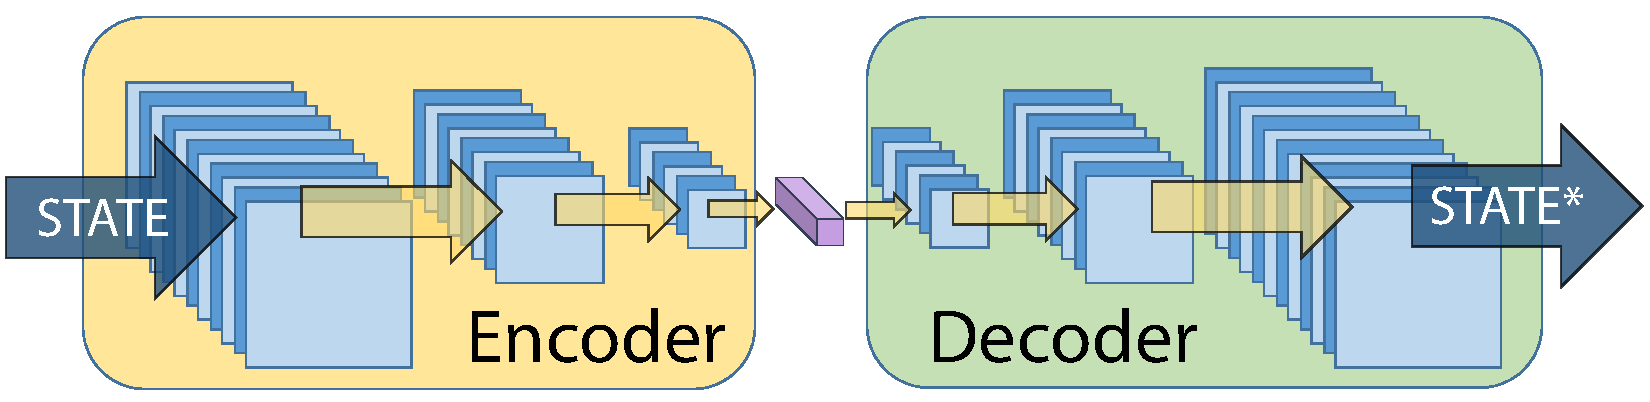
\includegraphics[width=0.45\linewidth]{imagenes/cap2/m1_p1.pdf}}
\hspace{0.1cm}
\subfloat[][Interactive training of the policy using the trained convolutional layers.]{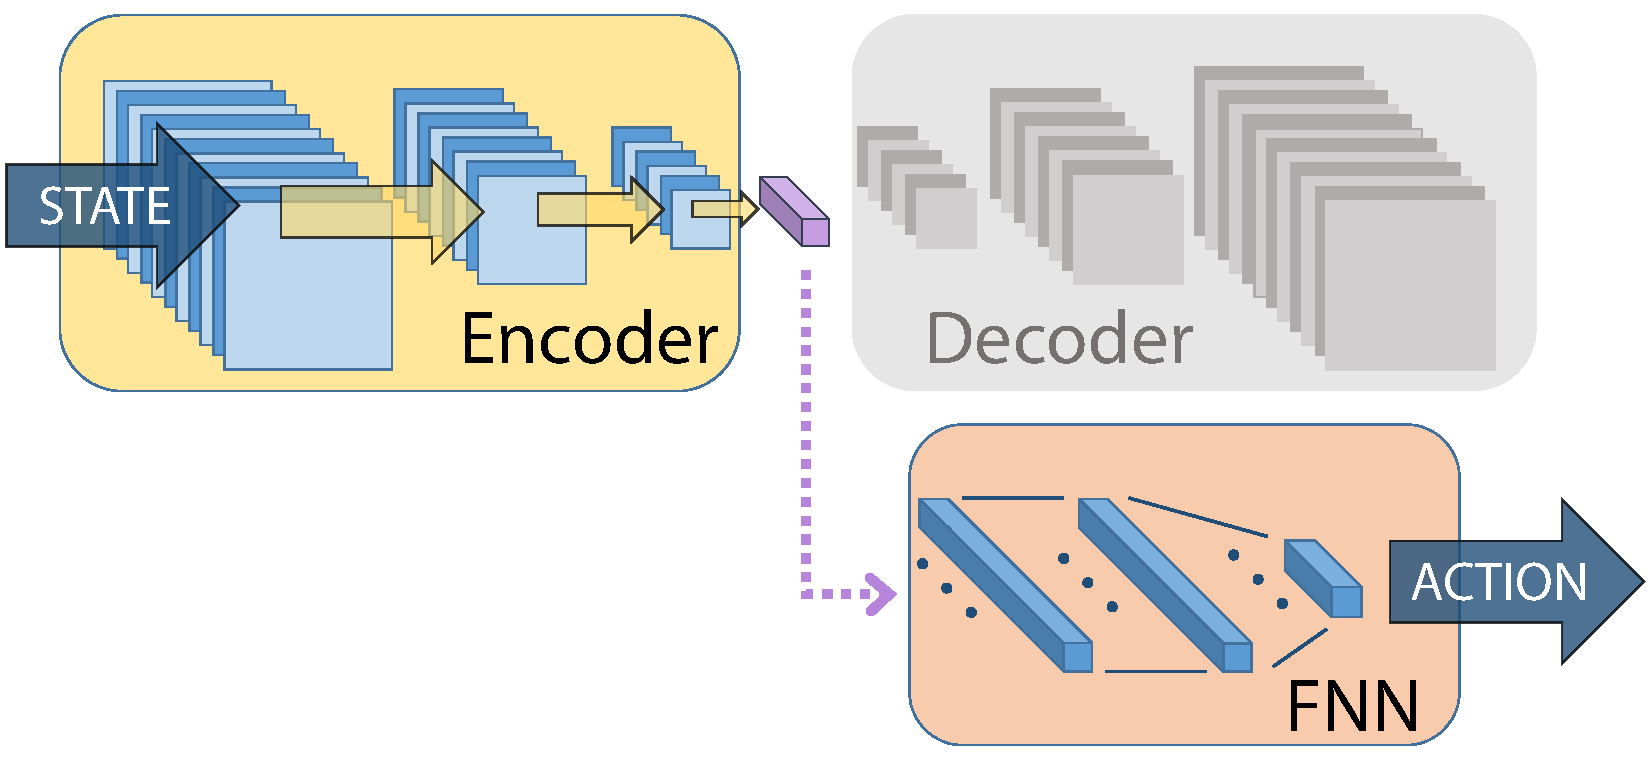
\includegraphics[width=0.45\linewidth]{imagenes/cap2/m1_p2.pdf}}
\caption{D-COACH offline state representation learning.} 
\label{fig:ms} 
\end{figure}

In the case of low-dimensional state problems, the state is fed into a FNN, skipping the autoencoder related steps and training the policy with interactive feedback directly. Figure \ref{fig:network_diagram} summarizes the network architecture for both low-dimensional and high-dimensional state problems.

\begin{figure}[h]
    \centering
    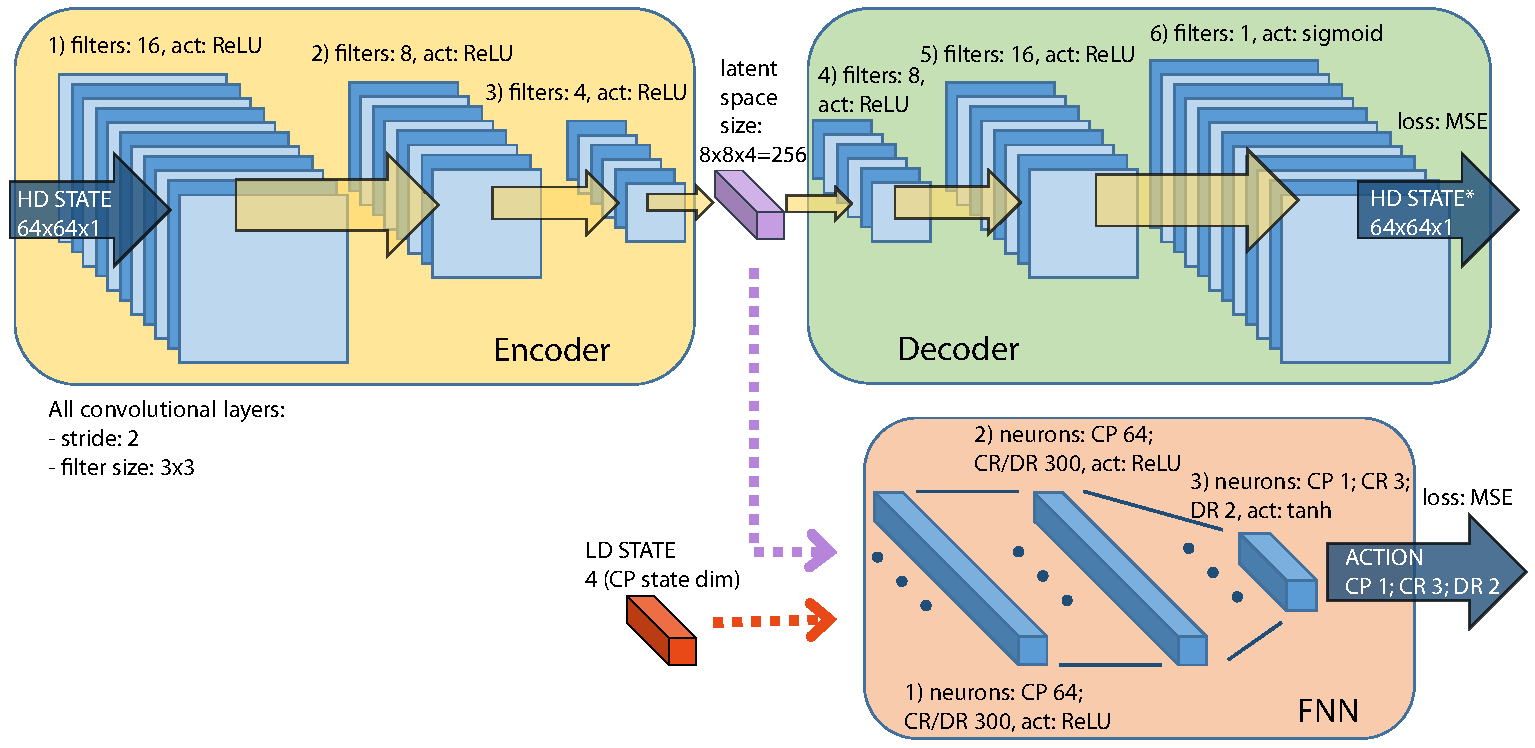
\includegraphics[width=0.9\linewidth]{imagenes/cap2/ISER_diagram.pdf}
    \caption{D-COACH neural networks architecture. HD STATE: high-dimensional state space, input of FNN is the latent space of the autoencoder (purple arrow). LD STATE: low-dimensional state space, input of FNN is the observed state (red arrow). Variations between environments are specified with the acronyms CP (Cart-Pole), CR (Car Racing) and DR (Duckie Racing). }
    \label{fig:network_diagram}
\end{figure}

\subsection{The Algorithm}
In D-COACH v1, the policies are updated every time feedback is received and also by sampling from a memory buffer $\mathcal{B}$ with a fixed frequency every $b$ time steps. Every time the user advises a correction, the buffer $\mathcal{B}$ is fed with the current state and a label generated by adding the action taken with the error correction $y_{label}=a+\mathit{error}$.

The high-dimensional case can be seen as an extension of the low-dimensional case, where an offline state learning process must be added. Algorithm \ref{algorithm:DeepCOACH} presents the D-COACH v1 pseudocode.

\begin{algorithm}[h]
\caption{D-COACH v1: Offline State Representation Learning}\label{algorithm:DeepCOACH}
\begin{algorithmic}[1]
\State \textbf{Require:} error magnitude $e$, buffer update interval $b$, buffer sampling size $N$, buffer min. size $k$, buffer max. size $K$, pre-trained encoder parameters (if convolutional) 
\State \textbf{Init:} $\mathcal{B} = []$  \emph{\# initialize memory buffer}
\For{t = 1,2,...}{}
\State \textbf{observe} state $s_{t}$
\State \textbf{execute} action $a_{t}=\pi(s_{t})$
\State \textbf{feedback} human corrective advice $h_{t}$
\If{$h_{t}$ is not \textbf{0}}
\State $\mathit{error}_{t} = h_{t}\cdot e$
\State $y_{label(t)} = a_{t} + \mathit{error}_{t}$ 
\State \textbf{update} $\pi(s)$ using SGD with pair ($s_{t}$, $y_{\mathit{label}(t)}$) 
\State \textbf{update} $\pi(s)$ using SGD with a mini-batch sampled from $\mathcal{B}$
\State \textbf{append} $(s_{t}, y_{\mathit{label}(t)})$ to $B$
\If{length($\mathcal{B}$) $> K$ }
\State $\mathcal{B} = \mathcal{B}[2:K+1]$
\EndIf
\EndIf
\If{mod(t, b) is 0 and length($\mathcal{B}$) $\geq k$}
\State \textbf{update} $\pi(s)$ using SGD with a mini-batch sampled from $\mathcal{B}$
\EndIf
\EndFor
\end{algorithmic}
\end{algorithm}

\section{Experiments and Results}
%\textbf{Even though COACH works well in low-dimensional state problems, the set of basis functions used in the LCBF must be selected independently for every problem. In some cases this could be time consuming or tedious. This engineering step is not necessary when using DNNs; thus, the same DNN architecture could be reused in different problems, saving time to the designers/engineers.}

Our proposed algorithm is validated experimentally in three different problems: 

\textbf{(i) Cart-Pole:} A simulated task with low-dimensional state space where the objective is to balance a pole attached to a cart. The cart can only move in one axis with an acceleration value between $-1$ and $1$. The state has four dimensions, which consists of the position $x$ and velocity $\dot x$ of the cart, and the angle $\theta$ and angular velocity $\dot \theta$ of the pole.

\textbf{(ii) Car Racing:} A simulated problem (from OpenAI gym \cite{brockman2016openai}) in which the agent has to learn to drive from a top-down view of a racing car game (see Fig.~\ref{fig:Car_Racing}). The objective of the task is to drive a racetrack as fast as possible without leaving it. The default state that is given by the environment is a $96\times96\times3$ top-down view of the car which we downsampled to $64\times64\times1$. The continuous-action space consists of 3 dimensions: \textbf{[direction, acceleration, brake]}. The \emph{direction} range goes from $-1$ to $1$, the \emph{acceleration} from $0$ to $1$ and the \emph{brake} from $0$ to $1$.

\begin{figure}[h]
    \centering
    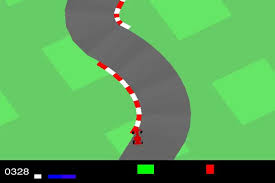
\includegraphics[scale=0.8]{imagenes/cap3/car_racing_env.jpg}
    \caption{Car Racing, environment view.}
    \label{fig:Car_Racing}
\end{figure}

\textbf{(iii) Duckie Racing:} This is also a driving task with high-dimensional input, but in this case with a real robot, which has an onboard camera that gives a first-person view of the environment. The robot consist of a Duckiebot from the project Duckietown \cite{Paull2017}. A $120\times160\times3$ observation image is received from the environment which is downsampled to $64\times64\times1$. The duckiebot is a differential robot, so the default actions consisted of speed commands ranging from -1 to 1 for each of the two wheels. To make it more intuitive for a human teacher to give feedback, the environment had an inverse kinematics module for the actions to be linear and rotational speeds instead, also ranging from -1 to 1. This problem is also used for experiments and validation with simulated and real human teachers.

The experiments with the simulated agents are intended to compare the complete D-COACH v1 presented in Algorithm \ref{algorithm:DeepCOACH}, along with a version of it without replay buffer (ignoring lines 2 and 11-16), and with a well known DRL agent (Deep Deterministic Policy Gradient DDPG \cite{Lillicrap2015} implemented by OpenAI \cite{baselines}). The comparison is carried out by plotting the cumulative reward obtained at each episode by the agent as a function of time. In the case of $\text{D-COACH}$ v1, the obtained reward is only used as a performance metric. Also, the results are presented as a function of time instead of episodes (except in the Duckie Racing experiment), because episodes can have variable duration depending on the policy. Hence, the episode scale would not properly show the time taken by the learning process, which is an important characteristic, since $\text{D-COACH}$ v1 is meant to work with real robots. The simulated environments, Cart-Pole and Car Racing, were ran at $22.5$ and $20.5$ FPS, respectively. These experiments were carried out using human teachers and simulated teachers. Humans had approximately 5 minutes to practice teaching in each environment. The learning curves of agents trained by 10 human teachers were obtained and averaged; the learning curves of agents trained by a simulated teacher were repeated 30 times and averaged. Along with the algebraic mean, the confidence intervals that represent the $60^{th}$ percentile of the data were plotted. In the case of the Car Racing problem, it was observed that coupled training was advantageous when the teachers were humans. The designed coupled signals are shown in Table \ref{table:coupled_car_racing}.

\begin{table}[t]
\centering
\caption{Values of $h$ in the Car Racing problem for human teachers. When feedback is given, the generated correction acts over more than one dimension of the action. For instance, the feedback signal \emph{forward} means that the agent should simultaneously increase its acceleration and decrease its brake.}
\label{table:coupled_car_racing}
\begin{tabular}{lc}
\textbf{Feedback            } & \multicolumn{1}{l}{          }{\textbf{h
(direction, acceleration, brake)}} \\ \hline \hline
Forward     & (0, 1, -1)                                       \\ \hline
Back        & (0, -1, 1)                                       \\ \hline
Left        & (-1, -1, 0)                                      \\ \hline
Right       & (1, -1, 0)                                       \\ \hline
\end{tabular}
\end{table}

The hyper-parameters of the neural networks used in these experiments were tuned with preliminary experiments. Different combinations of them were tested by a human teacher and the ones that made the training easiest were selected (see \figurename~{\ref{fig:network_diagram}}). The D-COACH error magnitude constant $e$ was set to $\textbf{1}$ in these experiments.

\subsection{Validation of replay buffer with simulated teachers}
The use of experience replay has been extensively validated in DRL; however, in this approach, we  still consider it necessary to test its impact. Unlike DRL, where the policy is updated with information collected from every time step, in COACH-like methods there is only new data to update the policy when feedback is given by the teacher, so the amount of data used to update the policy may be lower than in the RL case. Since the original COACH has been widely validated with real human teachers in several tasks, we carried out most of the comparisons using  a simulated teacher (a high performance policy standing-in as teacher, which was actually trained with D-COACH and a real human teacher) in this work, like in some of the experiments presented in \cite{Celemin2018AnInteractive}, in order to compare the methods under more controlled conditions. 

The simulated teacher generates feedback using $h = \operatorname{sign}(a_{\mathit{teacher}} - a_{\mathit{agent}})$, whereas the decision of advising feedback at each time step is given by the probability $P_{h} = \alpha \cdot\exp(-\tau\cdot \mathit{timestep})$, where $\{\alpha \in {\rm I\!R}\ | 0 \le \alpha \le 1\}$ and $\{\tau \in {\rm I\!R}\ | 0 \le \tau\}$. Additionally, since human teachers occasionally advise wrong corrections, a probability of giving erroneous feedback $P_{\mathit{err}}$ is added to the model. The variable $P_{\mathit{err}}$ indicates the probability that at least one dimension of $h$ is multiplied by $-1$ when feedback is given.

A comparison of D-COACH v1 with and without the use of an experience replay buffer is carried out by means of the simulated teacher. To test the behavior of these scenarios when erroneous feedback is added, different values of $P_{\mathit{err}}$ are selected. These results can be seen in \figurename~{\ref{fig:buffer_cart_pole}} and \figurename~{\ref{fig:buffer_car_racing}} (for better readability, no confidence intervals were added).

\begin{figure}[t]
    \centering
    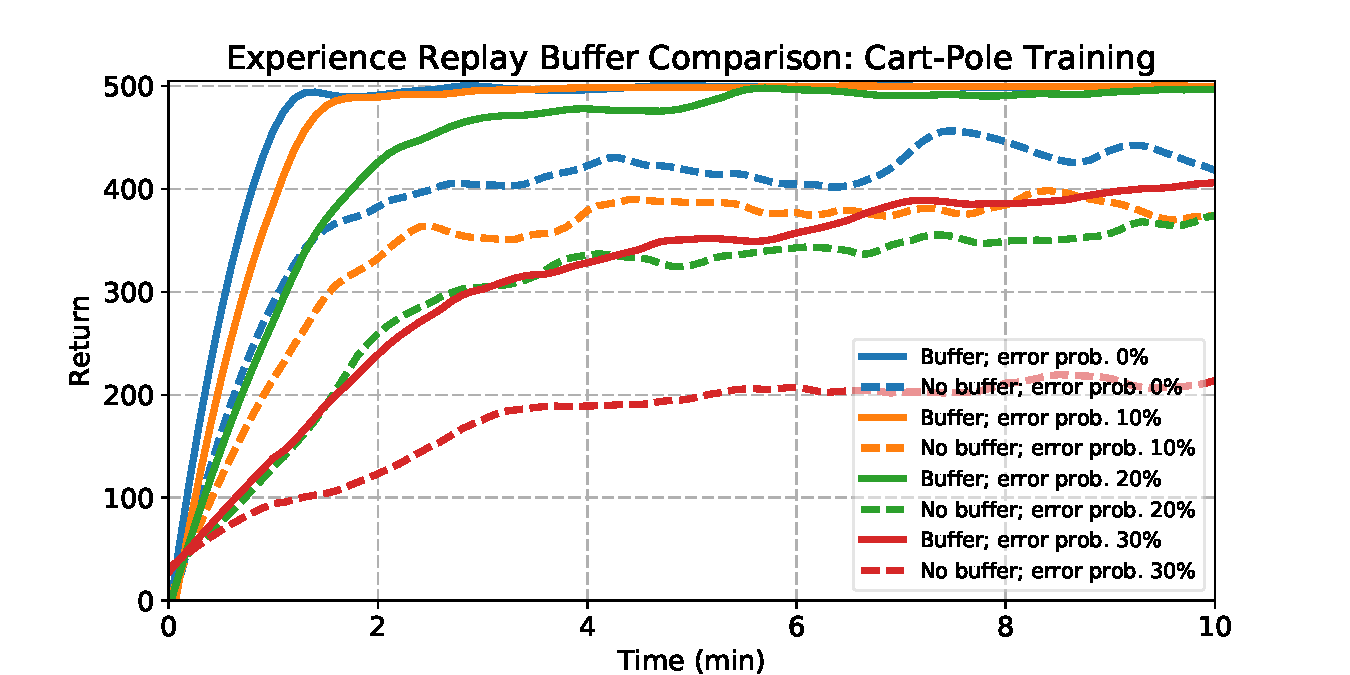
\includegraphics[width=0.9\linewidth]{imagenes/cap3/buffer_cart_pole.pdf}
    \caption{Comparison between using or not experience replay buffer for different values of $P_\mathit{err}$ in the Cart-Pole problem. Buffer: $K = 200$; $b = 10$; $N = 50$. $P_{h}$: $\alpha = 0.6$; $\tau = 0.0003$. Simulated teacher network learning rate: $0.0003$.}
    \label{fig:buffer_cart_pole}
\end{figure}

\begin{figure}[t]
    \centering
    \vspace{-0.2cm}
    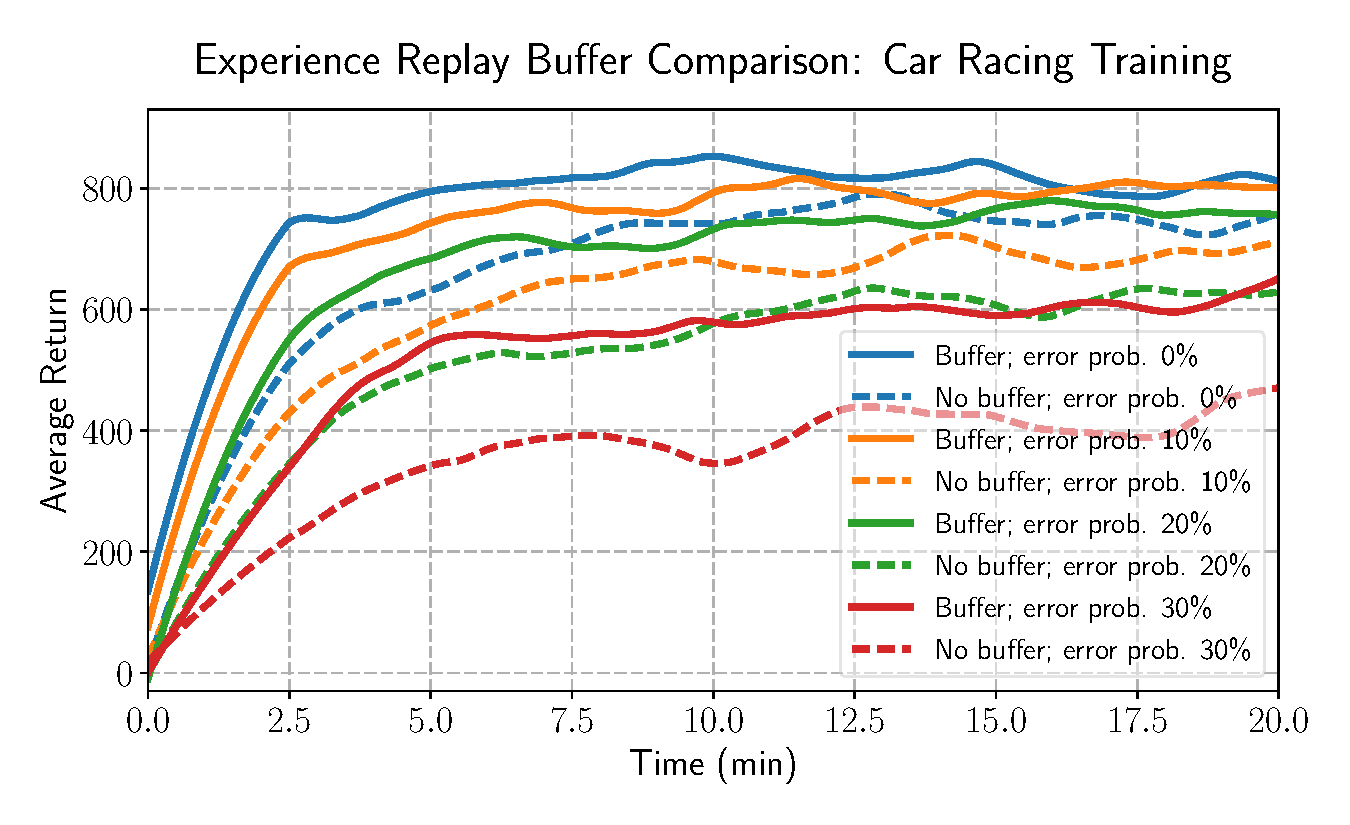
\includegraphics[width=0.9\linewidth]{imagenes/cap3/bufferCarRacing.pdf}
    \vspace{-0.2cm}
    \caption{Comparison between using or not experience replay buffer for different values of $P_\mathit{err}$ in the CarRacing problem. Buffer: $K = 1000$; $b = 10$; $N = 100$. $P_{h}$: $\alpha = 0.6$; $\tau = 0.000015$. Simulated teacher network learning rate: $0.0003$.}
    \label{fig:buffer_car_racing}
\end{figure}

In \figurename~{\ref{fig:buffer_cart_pole}} and \figurename~{\ref{fig:buffer_car_racing}} the learning curves show a large difference between the processes of learning that use experience replay buffer with respect to the cases without the buffer. In the case without the buffer, which is more similar to the original COACH, it is possible to see that the learning agent is not benefiting from the advised corrections as much as it can do when the pieces of advice are kept in the memory. For instance, we can see that $\text{D-COACH}$ v1 learns more from corrections with $20 \%$ of mistakes when using the buffer than in the case of perfect corrections, but without any buffering. This means the buffer is necessary for increasing the use of the available information, even when this information could be corrupted and not clean.

\subsection{Comparison of DRL and D-COACH using real human teachers}
\begin{figure}[t]
    \centering
    \vspace{-0.2cm}
    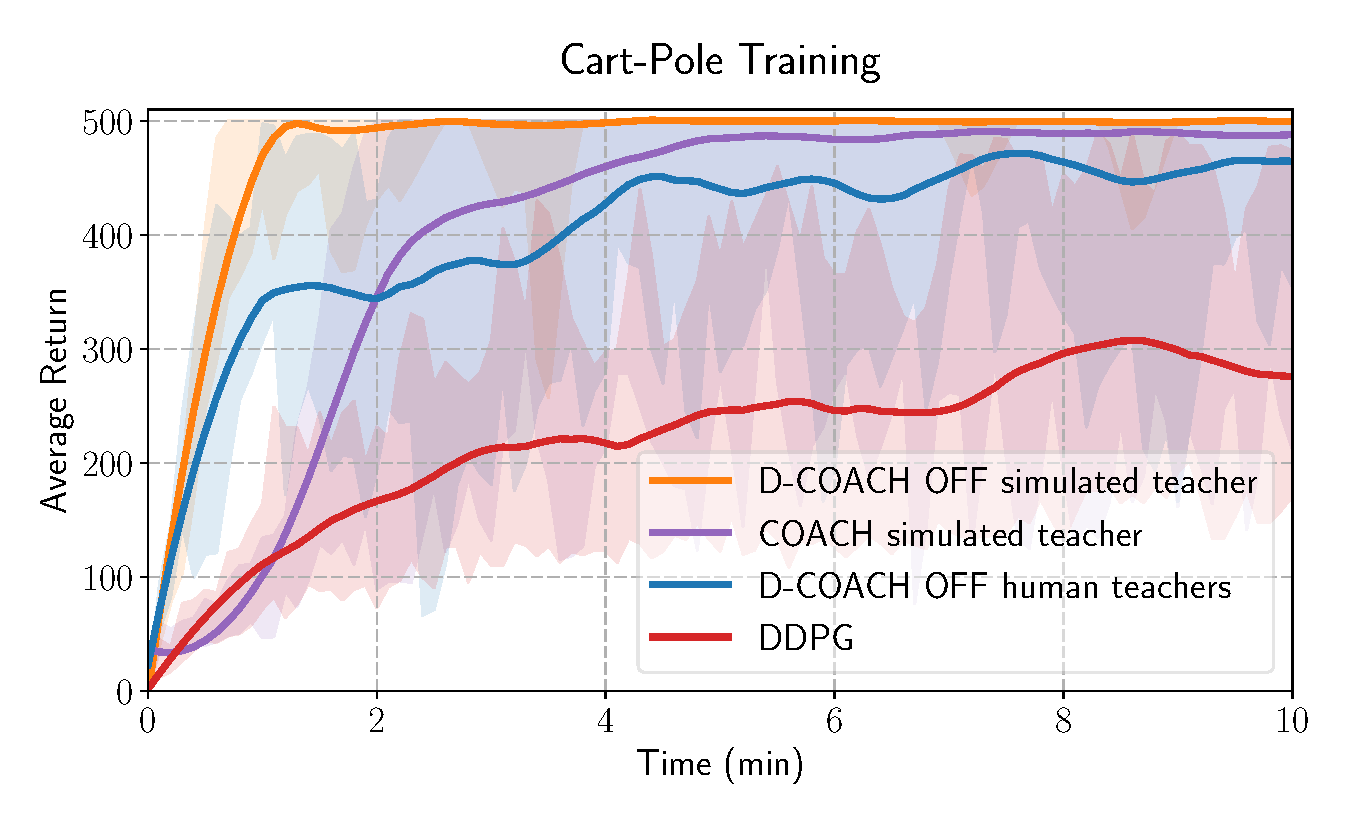
\includegraphics[width=0.9\linewidth]{imagenes/cap3/offline_cart_pole_humans.pdf}
    \vspace{-0.2cm}
    \caption{Cart-Pole training. Buffer: $K = 200$; $b = 10$; $N = 50$. $P_{h}$: $\alpha = 0.6$; $\tau = 0.0003$. Human teacher network learning rate: $0.003$; Simulated teacher network learning rate: $0.0003$.}
    \label{fig:cartpole_results}
\end{figure}

These experiments are intended to compare the learning process of D-COACH (simulated teacher and human teacher) with the DRL algorithm DDPG. Taking into account that the Cart-Pole problem has a low dimensional state space, the original COACH, based on basis functions, is also included in the comparison. In this case, $P_\mathit{err}=0\%$ was used for the simulated teachers. The results of this problem are shown in \figurename~{\ref{fig:cartpole_results}}, wherein it is possible to see that COACH-like methods outperform the DRL agent with a large difference. When using the simulated teacher, D-COACH v1 learns faster than the original COACH. The performance of D-COACH v1 with human teachers decreases with respect to the simulated teacher. This is because human teachers are not perfect and make mistakes, but they are being compared with a simulated teacher with $P_\mathit{err}=0\%$, which means that it makes no mistakes. Also because the simulated teacher model is quite simple to represent the complexity of the human behavior, then, although it is not very realistic, it is still useful for comparisons of interactive learning strategies under similar conditions.

In \figurename~{\ref{fig:racing_car_results1}} the learning curves of the Car Racing problem are presented. Again, D-COACH v1 results in a fast convergence. Unlike reported results of DRL algorithms for this problem, in the very early minutes D-COACH v1 reaches high performance policies that have not been obtained by most of the DRL approaches, to the best of our knowledge. If we compare a policy trained with D-COACH v1 for approximately 75 minutes by an experienced teacher against several state-of-the-art DRL approaches, it can be seen that it outperforms most of them (see Table \ref{CarRacing_table}). The problem is considered to be solved if the agent gets an average score of 900 or more over 100 random tracks. However, we observed that this value can substantially vary between different evaluations, so in Table \ref{CarRacing_table}, the obtained range of values over 20 evaluations is presented for D-COACH v1.
\vspace{-0.4cm}

\begin{figure}[t]
    \centering
    \vspace{-0.2cm}
    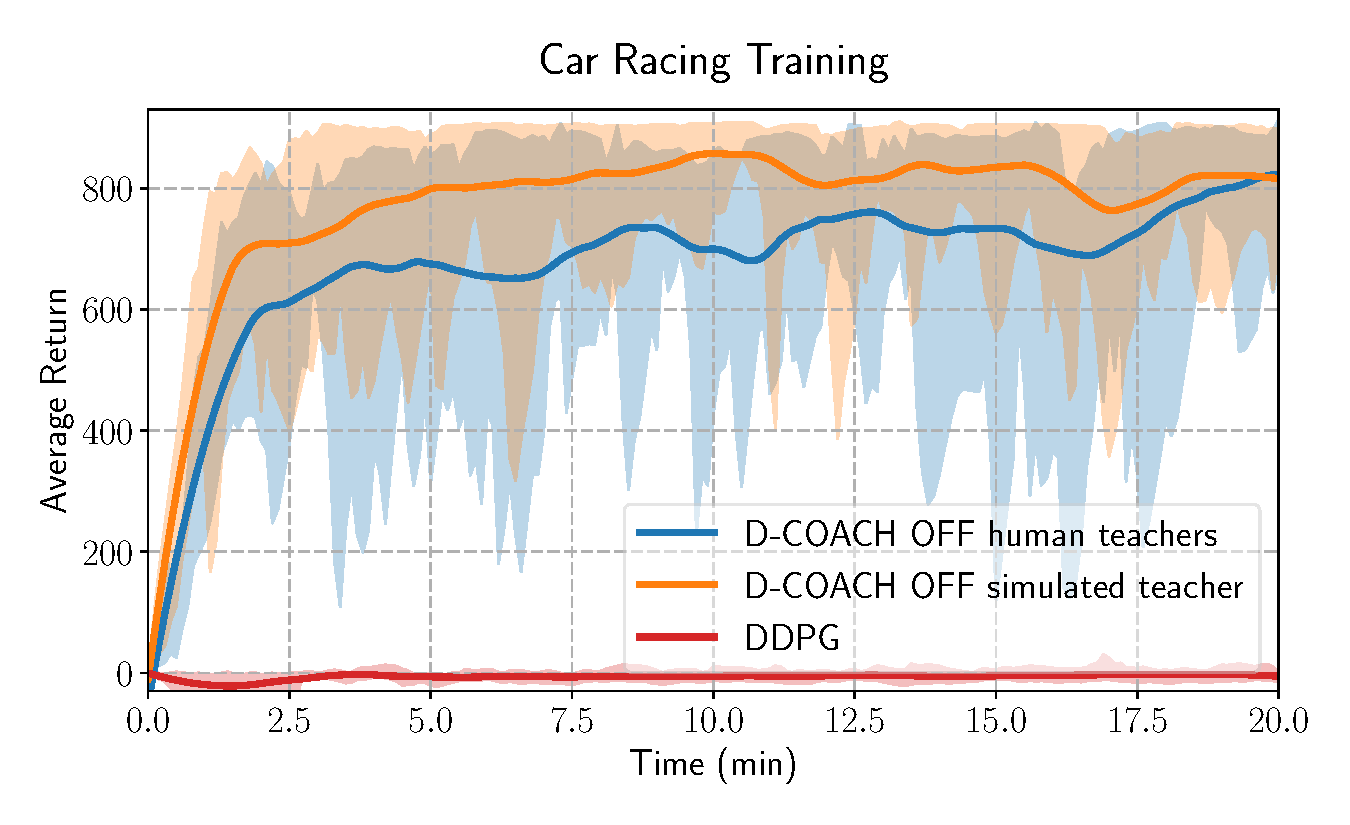
\includegraphics[width=0.9\linewidth]{imagenes/cap3/offline_car_racing_humans.pdf}
    \vspace{-0.2cm}
    \caption{Racing Car training. Buffer: $K = 1000$; $b = 10$; $N = 100$. $P_{h}$: $\alpha = 0.6$; $\tau = 0.000015$. Human teacher network learning rate: $0.001$; Simulated teacher network learning rate: $0.0003$.}
    \label{fig:racing_car_results1}
\end{figure}

\begin{table}[t]
\centering
\caption{Car Racing state-of-the-art learning algorithms comparison. DRL results taken from \cite{Ha2018}.}
\label{CarRacing_table}
\begin{tabular}{lc}
\multicolumn{1}{c}{\textbf{Method}}      & \multicolumn{1}{l}{\textbf{Average Score over 100 Random Tracks}} \\ \hline\hline
DQN                                      & 343 $\pm$ 18                                                      \\ \hline
A3C (continuous)                         & 591 $\pm$ 45                                                      \\ \hline
A3C (discrete)                           & 652 $\pm$ 10                                                      \\ \hline
ceobillionaire’s algorithm (unpublished) & 838 $\pm$ 11                                                      \\ \hline
Full World Model                         & 906 $\pm$ 21                                                      \\ \hline
\textbf{D-COACH (experienced teacher)}                         & \textbf{895 - 909 $\pm$ 18 - 80} \\
& \textbf{Average over 20 evaluations: 903 $\pm$ 46}
\\ \hline
\end{tabular}
\end{table}

\subsection{Validation in a real system}
In the third problem that we called Duckie Racing, an agent has to learn to drive a Duckiebot (from the project  Duckietown \cite{Paull2017} with modifications from the Chile Duckietown Team\footnote{\url{https://github.com/Duckietown-Chile/}}) autonomously through a track based on raw visual information of an onboard camera. The actions in this problem are the forward speed and the steering angle of the Duckiebot. Two tasks are set for this environment: (i) driving the Duckiebot freely through the track, with permission to drive in both lanes, and (ii) driving the Duckiebot only in the right lane, which demands more accuracy in driving. In this problem, an episode stops if the robot leaves the track/right lane, or after 30 seconds. The performance index in this task is the percentage of the total track length traveled during the episode. Hence the faster and more accurate the Duckiebot drives, the more distance it will travel.

This problem is not used for comparisons of the methods, but only as a validation of D-COACH using experience replay, which showed to be the best alternative in the previous problems. \figurename~\ref{fig:racing_duckie_results} shows the learning curve for each of the tasks explored in this environment with a real robot and a real human teacher. The curves and a video\footnote{https://youtu.be/vcEtuRrRIe4} attached to this thesis show that the system quickly learns to drive properly through the road based only on the human corrections. As expected, the policy is faster when the robot has the freedom to drive over both lanes. Learning this task with RL would definitely take more training time, and might need an external perception system to compute the reward function, whereas with D-COACH this performance index does not have any influence on the learning process, rather it is used for descriptive and comparative purposes.

\begin{figure}[H]
    \centering
    \begin{minipage}{.5\textwidth}
    \vspace{-0.2cm}
    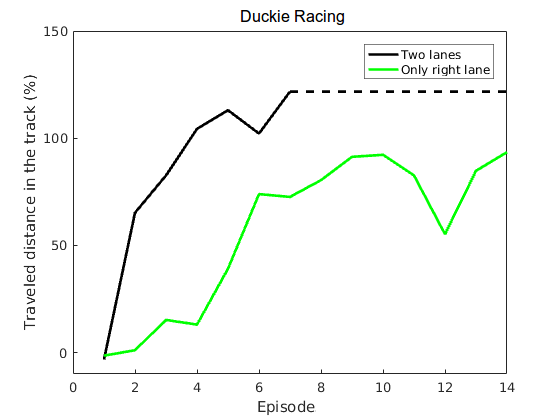
\includegraphics[width=1.0\linewidth]{imagenes/cap3/racing_duckie_results.png}
    \vspace{-0.2cm}
    \caption{Duckie Racing training.}
    \label{fig:racing_duckie_results}
    \end{minipage}%
    \begin{minipage}{.5\textwidth}
    \centering
    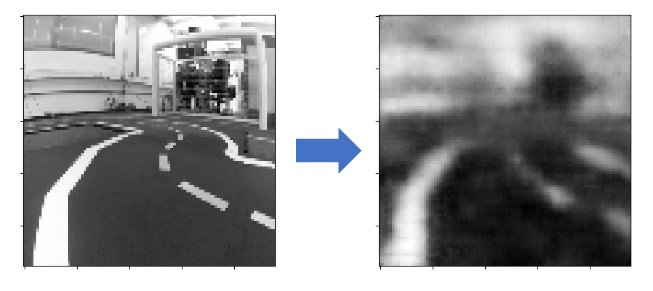
\includegraphics[width=1.0\linewidth]{imagenes/cap3/AE_duckie2.png}
    \vspace{-0.2cm}
    \caption{Duckie Racing autoencoder input (left) vs output (right).}
    \label{fig:AE_duckie}
    \end{minipage}
\end{figure}

\section{Discussion}
This chapter presented D-COACH v1, an algorithm for training policies modeled with DNNs interactively with corrective advice. The method was validated in a problem of low-dimensionality, along with problems of high-dimensional state spaces like raw pixel observations, with a simulated and a real robot environment, and also using both simulated and real human teachers. 

The use of the experience replay buffer (which has been well tested for DRL) was re-validated for this different kind of learning approach, since this is a feature not included in the original COACH. The comparisons showed that the use of memory resulted in an important boost in the learning speed of the agents, which were able to converge with less feedback, and to perform better even in cases with a significant amount of erroneous signals.  

The results of the experiments show that teachers advising corrections can train policies in fewer time steps than a DRL method like DDPG. So it was possible to train real robot tasks based on human corrections during the task execution, in an environment with a raw pixel level state space. 

The comparison of D-COACH with respect to DDPG, shows how this interactive method makes it more feasible to learn policies represented with DNNs, within the constraints of physical systems. DDPG needs to accumulate millions of time steps of experience in order to obtain good performances as shown in \cite{Lillicrap2015}. However, this is not always possible with real systems.
\begin{conclusion}
We presented a framework for learning continuous-action policies using corrective feedback to shape DNN policies in high and low dimensional state spaces. This work was inspired in the COrrective Advice Communicated by Humans (COACH) framework, from where two ideas were taken: (1) the use of binary corrective feedback in action spaces for shaping policies, and (2) the use of past corrections to modify the effects of newer ones. In the COACH framework, these ideas were validated in problems with low-dimensional state spaces using linear combination of basis functions (LCBFs) as function approximators. The novelty of this work is that Deep Neural Networks (DNNs) were used instead, combining ideas of the Deep Reinforcement Learning (DRL) era with the ones of COACH, creating Deep COACH (D-COACH). With D-COACH, we showed that by combining Deep Learning with COACH it is possible to extrapolate the ideas of COACH to learn policies in high-dimensional state spaces and in Partially Observable Markov Decision Processes (POMDPs) within the tens of minutes. 

The hypothesis of this thesis was supported with several experiments. We showed that human corrective feedback can be used to learn well performing DNN policies in a time-efficient and reward function free way.

First, D-COACH was validated in a low-dimensional state problem (cart-pole). This is a simple widely-studied problem that is useful to test early versions of sequential decision making learning algorithms. This problem had also been previously solved using COACH, which made it a good candidate to compare the performance of D-COACH with the one of COACH. This experiment showed that D-COACH worked well in low-dimensional state problems and with a performance similar to the one of COACH. 

For high-dimensional state problems, two variations of D-COACH were proposed and compared: online state learning and offline state learning. Both variations obtained similar final performances in the Car Racing and the Duckie Racing problems. The main advantage found in the online state learning version over the offline state version, is that it is an approach that requires less time and effort from the human user. Everything is learned from scratch and interactively, while in the offline state learning case a database of the agent exploring the environment must be obtained and used to train an autoencoder before starting the interactive learning process of the policy. Online state learning D-COACH had an extra validation in a 3DoF arm, where an agent learned to solve the reacher and pusher tasks from scratch.

Finally, a last variation of D-COACH (model-based) for POMDPs in where the observations do not capture time-dependent phenomena from the state was proposed. The approach was to give memory to the agent by adding recurrent layers, LSTMs, to the DNN models. By comparing model-free with model-based D-COACH in low and high dimensional state problems using a simulated teacher, we observed that learning a model of the dynamics of the environment could be crucial in some cases for obtaining well performing policies. Also, that in other cases it may improve the performance of the agent. 

Even though the algorithms proposed in this work were validated and supported the hypothesis of this thesis, we believe that there is still a lot of work and research left to be done in this area. There are some ideas proposed in the COACH framework that we did not study with D-COACH and are worth mentioning:

\begin{itemize}
    \item \textbf{Human Model:} In D-COACH we replaced the Human Model with a replay buffer, as mentioned in Chapter 2. Even though both approaches use information given by past corrections to modify the effects of newer ones, they do not do it in the same way. The Human Model modifies the learning rate of the policy; the replay buffer updates the policy constantly by replaying past corrections. Including a Human Model in D-COACH could help with the dilemma of setting either a too large or too small magnitude of the learning rate when updating the policy with SGD. In this case, we did not include a Human Model because this would have meant to add a second DNN model in charge of learning it. Thus, the overhead of D-COACH would have increased and for a first approach we prioritized a lighter model.
    \item \textbf{Credit assigner:} Module proposed in TAMER approaches \cite{Knox:2009:ISA:1597735.1597738} which COACH adopted. This module associates feedback not only with the last state-action pair, but with past state-action pairs as well. The objective is to characterize the the human delay with a probability that weights correction signals with a sequence of state-action pairs. This could help with the data-efficiency of D-COACH. Nevertheless, given that D-COACH was able to work fine without this module, studying the advantages of adding it to the framework was left for future work. 
    \item \textbf{D-COACH + DRL:} In \cite{celemin2018fast}, a hybrid RL framework with COACH is proposed. The basic idea is to use corrective feedback along with RL algorithms in order to speed up the learning process. The same concept could be applied and studied with D-COACH. 
\end{itemize}

In contrast, the are some shortcomings that D-COACH presents that would be beneficial to study in future research:
\begin{itemize}
    \item \textbf{High-dimensional action spaces:} One of the main shortcomings of D-COACH was inherited from COACH. Both approaches are limited to work in problems with low-dimensional action spaces due to that humans must provide corrections in the action space. If the action space of a problem is too large, then is not intuitive for a human to give feedback, and he/she may not be able to correct the agent. Modules that interpret feedback from a correction space to the agent's action space can be added to tackle this shortcoming, such using inverse kinematics modules. But this is not always possible or trivial to do, so more research in this area could  enhance the capabilities of D-COACH.
    \item \textbf{Experience Replay size:} Given that the size of the replay buffer of D-COACH is limited due to its on-policy nature, it may be challenging (or not possible) to solve problems that require more complex decision-making strategies that the ones tested in this thesis. This is because in more complex scenarios, agents may need to store corrections in memory for a longer time than what the buffer is able to do, due to its limited size. Thus, valuable corrections would be forgotten, affecting the performance of the agent. Developing strategies to overcame this limitation could be key for using D-COACH in more complex settings. 
\end{itemize}

Beyond the limitations of D-COACH and the future research that can be done in this area, the variations of D-COACH presented in this work showed to be a valid alternative for teaching robots to solve sequential decision-making problems using DNN policies. Human teachers were able to interact with real-world platforms (Duckie Racing and 3DoF arm) and guide them through the learning process for solving tasks.
\end{conclusion}


\nocite{*}
\bibliographystyle{plain}
\bibliography{bibliography}
\end{document}
